\documentclass[tikz,border=8pt]{standalone}
\usepackage{ctex}
\usepackage{amsmath,amssymb}
\usetikzlibrary{arrows.meta,calc,angles,quotes,patterns,positioning,decorations.pathmorphing}
\definecolor{ink}{RGB}{30,43,58}
\definecolor{blue}{RGB}{38,92,168}
\definecolor{orange}{RGB}{220,112,24}
\definecolor{green}{RGB}{38,139,93}
\definecolor{red}{RGB}{192,53,53}
\tikzset{
 line cap=round,line join=round,
 body/.style={draw=ink,very thick},
 axis/.style={-{Latex[length=2.5mm]},draw=ink,very thick},
 vec/.style={-{Latex[length=2.5mm]},draw=blue,very thick},
 force/.style={-{Latex[length=2.5mm]},draw=red,very thick},
 guide/.style={draw=ink!48,dashed},
 dim/.style={{Latex[length=2mm]}-{Latex[length=2mm]},draw=ink!70}
}

\usetikzlibrary{decorations.pathmorphing}
\tikzset{mass/.style={circle,draw,fill=white,minimum size=7mm},curve/.style={very thick,blue},rope/.style={very thick,blue},ray/.style={very thick,blue,-{Latex}},impulse/.style={very thick,orange,-{Latex}},current/.style={very thick,orange,-{Latex}},resistor/.style={thick,decorate,decoration={zigzag,segment length=3mm,amplitude=1mm}}}
\begin{document}
% 1 question-01
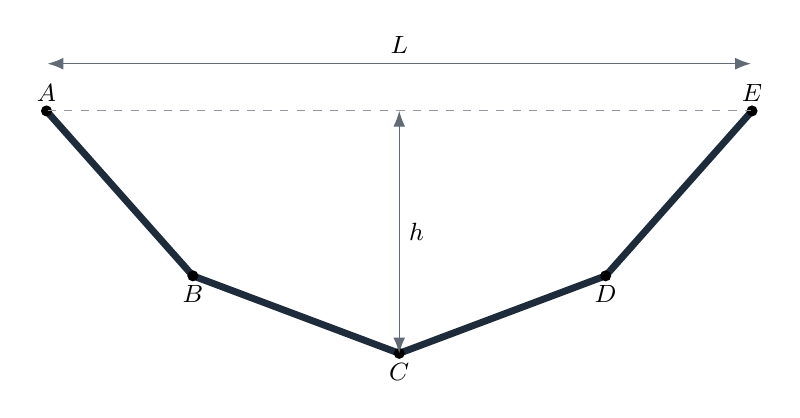
\begin{tikzpicture}[x=1cm,y=1cm,font=\small]
\draw[body,line width=2.5pt] plot coordinates {(-4.480000,0.000000) (-2.621261,-2.094060) (0.000000,-3.078434) (2.621261,-2.094060) (4.480000,0.000000)};
\fill (-4.480000,0.000000) circle(2pt) node[above] {$A$};
\fill (-2.621261,-2.094060) circle(2pt) node[below] {$B$};
\fill (0.000000,-3.078434) circle(2pt) node[below] {$C$};
\fill (2.621261,-2.094060) circle(2pt) node[below] {$D$};
\fill (4.480000,0.000000) circle(2pt) node[above] {$E$};
\draw[guide] (-4.466,0)--(4.466,0);\draw[dim] (-4.466,.6)--(4.466,.6) node[midway,above] {$L$};\draw[dim] (0,0)--(0,-3.078) node[midway,right] {$h$};
\end{tikzpicture}

% 2 solution-01
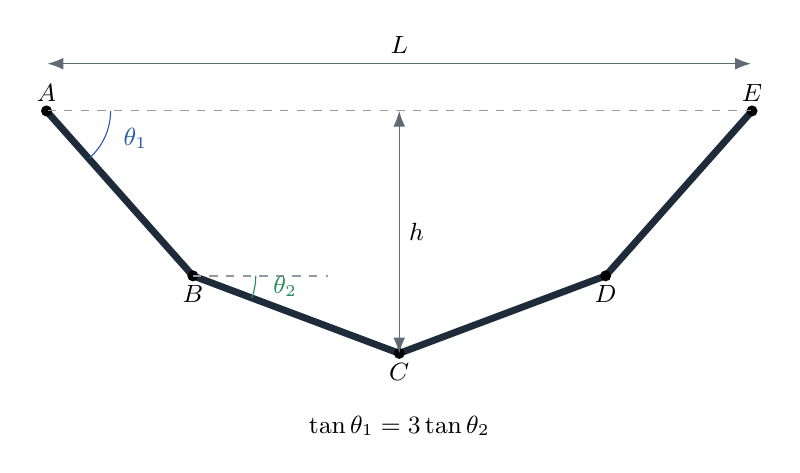
\begin{tikzpicture}[x=1cm,y=1cm,font=\small]
\draw[body,line width=2.5pt] plot coordinates {(-4.480000,0.000000) (-2.621261,-2.094060) (0.000000,-3.078434) (2.621261,-2.094060) (4.480000,0.000000)};
\fill (-4.480000,0.000000) circle(2pt) node[above] {$A$};
\fill (-2.621261,-2.094060) circle(2pt) node[below] {$B$};
\fill (0.000000,-3.078434) circle(2pt) node[below] {$C$};
\fill (2.621261,-2.094060) circle(2pt) node[below] {$D$};
\fill (4.480000,0.000000) circle(2pt) node[above] {$E$};
\draw[guide] (-4.466,0)--(4.466,0);\draw[dim] (-4.466,.6)--(4.466,.6) node[midway,above] {$L$};\draw[dim] (0,0)--(0,-3.078) node[midway,right] {$h$};\draw[guide] (-2.622,-2.096)--(-.9,-2.096);\draw[blue] (-4.466,0)++(0:.8) arc(0:-48.4:.8);\node[blue] at (-3.35,-.35) {$\theta_1$};\draw[green] (-2.622,-2.096)++(0:.8) arc(0:-20.57:.8);\node[green] at (-1.45,-2.23) {$\theta_2$};\node at (0,-4) {$\tan\theta_1=3\tan\theta_2$};
\end{tikzpicture}

% 3 question-02
\begin{tikzpicture}[x=1cm,y=1cm,font=\small]
\draw[axis] (-.3,0)--(8,0) node[right] {$x$};\draw[axis] (0,-.3)--(0,4.9) node[above] {$y$};\draw[body] (0,3.6)--(6.1,.078);\node at (5.5,1.2) {屋面};\draw[guide] (0,3.6)--(2,3.6);\draw[blue] (0,3.6)++(0:.9) arc(0:-30:.9);\node[blue] at (1.4,3.35) {$\alpha$};\draw[orange,very thick] plot coordinates {(0.000000,0.000000) (0.037343,0.026121) (0.074685,0.052187) (0.112028,0.078199) (0.149370,0.104157) (0.186713,0.130061) (0.224056,0.155911) (0.261398,0.181707) (0.298741,0.207449) (0.336083,0.233136) (0.373426,0.258770) (0.410768,0.284349) (0.448111,0.309874) (0.485454,0.335345) (0.522796,0.360762) (0.560139,0.386125) (0.597481,0.411434) (0.634824,0.436688) (0.672167,0.461889) (0.709509,0.487035) (0.746852,0.512127) (0.784194,0.537166) (0.821537,0.562150) (0.858880,0.587079) (0.896222,0.611955) (0.933565,0.636777) (0.970907,0.661544) (1.008250,0.686258) (1.045592,0.710917) (1.082935,0.735522) (1.120278,0.760073) (1.157620,0.784570) (1.194963,0.809013) (1.232305,0.833402) (1.269648,0.857736) (1.306991,0.882017) (1.344333,0.906243) (1.381676,0.930415) (1.419018,0.954534) (1.456361,0.978598) (1.493703,1.002607) (1.531046,1.026563) (1.568389,1.050465) (1.605731,1.074312) (1.643074,1.098106) (1.680416,1.121845) (1.717759,1.145530) (1.755102,1.169161) (1.792444,1.192738) (1.829787,1.216261) (1.867129,1.239729) (1.904472,1.263144) (1.941815,1.286504) (1.979157,1.309811) (2.016500,1.333063) (2.053842,1.356261) (2.091185,1.379405) (2.128527,1.402495) (2.165870,1.425531) (2.203213,1.448512) (2.240555,1.471440) (2.277898,1.494313) (2.315240,1.517132) (2.352583,1.539897) (2.389926,1.562609) (2.427268,1.585265) (2.464611,1.607868) (2.501953,1.630417) (2.539296,1.652911) (2.576639,1.675352) (2.613981,1.697738) (2.651324,1.720070) (2.688666,1.742348) (2.726009,1.764572) (2.763351,1.786742) (2.800694,1.808858) (2.838037,1.830919) (2.875379,1.852927) (2.912722,1.874880) (2.950064,1.896779)};
\fill (2.950064,1.896779) circle(2pt) node[above left] {$P$};
\draw[vec] (0,0)--(.819,.574) node[above] {$v_0$};
\end{tikzpicture}

% 4 solution-02
\begin{tikzpicture}[x=1cm,y=1cm,font=\small]
\draw[axis] (-.3,0)--(8,0) node[right] {$x$};\draw[axis] (0,-.3)--(0,4.9) node[above] {$y$};\draw[body] (0,3.6)--(6.1,.078);\node at (5.5,1.2) {屋面};\draw[guide] (0,3.6)--(2,3.6);\draw[blue] (0,3.6)++(0:.9) arc(0:-30:.9);\node[blue] at (1.4,3.35) {$\alpha$};\draw[orange,very thick] plot coordinates {(0.000000,0.000000) (0.037343,0.026121) (0.074685,0.052187) (0.112028,0.078199) (0.149370,0.104157) (0.186713,0.130061) (0.224056,0.155911) (0.261398,0.181707) (0.298741,0.207449) (0.336083,0.233136) (0.373426,0.258770) (0.410768,0.284349) (0.448111,0.309874) (0.485454,0.335345) (0.522796,0.360762) (0.560139,0.386125) (0.597481,0.411434) (0.634824,0.436688) (0.672167,0.461889) (0.709509,0.487035) (0.746852,0.512127) (0.784194,0.537166) (0.821537,0.562150) (0.858880,0.587079) (0.896222,0.611955) (0.933565,0.636777) (0.970907,0.661544) (1.008250,0.686258) (1.045592,0.710917) (1.082935,0.735522) (1.120278,0.760073) (1.157620,0.784570) (1.194963,0.809013) (1.232305,0.833402) (1.269648,0.857736) (1.306991,0.882017) (1.344333,0.906243) (1.381676,0.930415) (1.419018,0.954534) (1.456361,0.978598) (1.493703,1.002607) (1.531046,1.026563) (1.568389,1.050465) (1.605731,1.074312) (1.643074,1.098106) (1.680416,1.121845) (1.717759,1.145530) (1.755102,1.169161) (1.792444,1.192738) (1.829787,1.216261) (1.867129,1.239729) (1.904472,1.263144) (1.941815,1.286504) (1.979157,1.309811) (2.016500,1.333063) (2.053842,1.356261) (2.091185,1.379405) (2.128527,1.402495) (2.165870,1.425531) (2.203213,1.448512) (2.240555,1.471440) (2.277898,1.494313) (2.315240,1.517132) (2.352583,1.539897) (2.389926,1.562609) (2.427268,1.585265) (2.464611,1.607868) (2.501953,1.630417) (2.539296,1.652911) (2.576639,1.675352) (2.613981,1.697738) (2.651324,1.720070) (2.688666,1.742348) (2.726009,1.764572) (2.763351,1.786742) (2.800694,1.808858) (2.838037,1.830919) (2.875379,1.852927) (2.912722,1.874880) (2.950064,1.896779)};
\fill (2.950064,1.896779) circle(2pt) node[above left] {$P$};
\draw[vec] (0,0)--(.819,.574) node[above] {$v_0$};\draw[vec] (2.9500644,1.8967794642402387)--++(1.25,.732) node[right] {$\vec v$};\node[align=center] at (4,-1.0) {$\theta_{\rm opt}=\pi/2-\alpha$\\$y=h-x\tan\alpha$};
\end{tikzpicture}

% 5 question-03
\begin{tikzpicture}[x=1cm,y=1cm,font=\small]
\fill[blue!8] (-4,-1.5) rectangle(0,1.5);\draw[body] (0,-1.5)--(0,1.5);\fill[ink!8] (0,-1.5)--(1.11,-1.5) arc(210:150:3)--(0,1.5)--cycle;\draw[body] (1.11,-1.5) arc(210:150:3);\draw[axis] (-4.5,0)--(6.8,0) node[right] {光轴};\node at (-3,1.9) {水 $n_w$};\node at (.2,1.9) {玻璃 $n$};\node at (4.8,1.9) {空气};\draw[ray] (-4,-0.75)--(0.8032624903444376,-0.75)--(5.8,-1.686888283060418);\draw[ray] (-4,0.75)--(0.8032624903444376,0.75)--(5.8,1.686888283060418);\fill (3.708,0) circle(2pt) node[below] {$C$};\draw[dim] (.708,-1.9)--(3.708,-1.9) node[midway,below] {$R>0$};
\end{tikzpicture}

% 6 solution-03
\begin{tikzpicture}[x=1cm,y=1cm,font=\small]
\fill[blue!8] (-4,-1.5) rectangle(0,1.5);\draw[body] (0,-1.5)--(0,1.5);\fill[ink!8] (0,-1.5)--(1.11,-1.5) arc(210:150:3)--(0,1.5)--cycle;\draw[body] (1.11,-1.5) arc(210:150:3);\draw[axis] (-4.5,0)--(6.8,0) node[right] {光轴};\node at (-3,1.9) {水 $n_w$};\node at (.2,1.9) {玻璃 $n$};\node at (4.8,1.9) {空气};\draw[ray] (-4,-0.75)--(0.8032624903444376,-0.75)--(5.8,-1.686888283060418);\draw[guide] (0.8032624903444376,-0.75)--(-3.1,0);\draw[ray] (-4,0.75)--(0.8032624903444376,0.75)--(5.8,1.686888283060418);\draw[guide] (0.8032624903444376,0.75)--(-3.1,0);\fill (3.708,0) circle(2pt) node[below] {$C$};\draw[dim] (.708,-1.9)--(3.708,-1.9) node[midway,below] {$R>0$};\node at (0,-2.8) {$\Phi=(1-n)/R<0$，反向延长线给虚焦点};
\end{tikzpicture}

% 7 question-04
\begin{tikzpicture}[scale=1]
  \begin{scope}[xshift=-3.2cm]
    \draw[axis] (-2.5,0)--(3,0) node[right] {$z$};
    \fill[blue] (-.9,0) circle(3pt) node[above] {$-q_m$};
    \fill[red] (.9,0) circle(3pt) node[above] {$+q_m$};
    \draw[dim] (-.9,-.55)--(.9,-.55) node[midway,below] {$d$};
    \fill[ink] (2.55,0) circle(2.2pt) node[above] {$P(z)$};
    \node at (0,-1.7) {Gilbert 模型};
  \end{scope}
  \begin{scope}[xshift=3.3cm]
    \draw[axis] (-2.6,0)--(3,0) node[right] {$z$};
    \draw[body,fill=blue!8] (0,0) ellipse(.52 and 1.55);
    \draw[orange,very thick,-{Latex}] (0,1.55)
      arc[start angle=90,end angle=-120,x radius=.52,y radius=1.55];
    \node[orange] at (.9,1.25) {$I$};
    \draw[dim] (0,-1.85)--(.52,-1.85) node[midway,below] {$r$};
    \fill[ink] (2.55,0) circle(2.2pt) node[above] {$P(z)$};
    \node at (0,-2.55) {Ampere 模型};
  \end{scope}
\end{tikzpicture}

% 8 solution-04
\begin{tikzpicture}[x=1cm,y=1cm,font=\small]
\begin{scope}[xshift=-3.1cm]\draw[body,fill=blue!6] (-2,-.9) rectangle(2,.9);\draw[axis] (-2.4,0)--(2.6,0) node[right] {$z$};\node[red] at (2.1,-0.6) {$+$};\node[blue] at (-2.1,-0.6) {$-$};\node[red] at (2.1,0) {$+$};\node[blue] at (-2.1,0) {$-$};\node[red] at (2.1,0.6) {$+$};\node[blue] at (-2.1,0.6) {$-$};\draw[force] (.8,.35)--(-.8,.35) node[midway,above] {$B_G<0$};\node at (0,-1.55) {$B_G=-\mu_0M(1-a/\sqrt{a^2+R^2})$};\draw[dim] (-2,-2.1)--(2,-2.1) node[midway,below] {$L=2a$};\end{scope}\begin{scope}[xshift=3.1cm]\draw[body,fill=blue!6] (-2,-.9) rectangle(2,.9);\draw[axis] (-2.4,0)--(2.6,0) node[right] {$z$};\draw[orange,->] (-1.5,-.9) arc(270:90:.18 and .9);\draw[orange,->] (-0.75,-.9) arc(270:90:.18 and .9);\draw[orange,->] (0,-.9) arc(270:90:.18 and .9);\draw[orange,->] (0.75,-.9) arc(270:90:.18 and .9);\draw[orange,->] (1.5,-.9) arc(270:90:.18 and .9);\draw[vec] (-.8,.35)--(.8,.35) node[midway,above] {$B_A>0$};\node at (0,-1.55) {$B_A=\mu_0Ma/\sqrt{a^2+R^2}$};\draw[dim] (-2,-2.1)--(2,-2.1) node[midway,below] {$L=2a$};\end{scope}\node at (0,-3) {$B_A-B_G=\mu_0M$；辅助磁荷算的是 $H$};
\end{tikzpicture}

% 9 question-05
\begin{tikzpicture}[scale=1]
  \draw[body,line width=2pt,rounded corners=3pt] (-2.5,-2.6) rectangle (2.5,2.6);
  \fill[blue!22] (-2.35,-2.45) rectangle (2.35,-.65);
  \draw[blue,very thick] (-2.35,-.65)--(2.35,-.65);
  \node[blue] at (0,-1.55) {液态水 $1\,\mathrm{mol}$};
  \node at (0,.95) {饱和水蒸气 $1\,\mathrm{mol}$};
  \draw[orange,very thick,decorate,decoration={zigzag,segment length=5pt,amplitude=2pt}]
    (-1.2,.1)--(1.2,.1);
  \node[orange,right] at (1.25,.1) {电热丝};
  \node[red] at (0,3.05) {器壁绝热，$V=\text{常量}$};
\end{tikzpicture}

% 10 solution-05
\begin{tikzpicture}[scale=1]
  \node[draw=ink,very thick,rounded corners,fill=orange!10,minimum width=3.3cm,minimum height=1cm] (Q) at (0,2.3) {输入能量 $Q$};
  \node[draw=ink,very thick,rounded corners,fill=blue!9,align=center,minimum width=4.1cm,minimum height=1.2cm] (A) at (-3,-.2) {原有液体与蒸气升温\\$(C+3R)\Delta T$};
  \node[draw=ink,very thick,rounded corners,fill=green!10,align=center,minimum width=4.1cm,minimum height=1.2cm] (B) at (3,-.2) {少量液体汽化\\$\Delta n(L-RT_0)$};
  \draw[vec] (Q)--(A); \draw[vec] (Q)--(B);
  \node[align=center] at (0,-2.15)
   {$\displaystyle \Delta n=\frac{n_0\Delta T}{T_0}
   \left(\frac{L}{RT_0}-1\right)$\\[5pt]
    $Q=(C+3R)\Delta T+\Delta n(L-RT_0)$};
\end{tikzpicture}

% 11 question-06
\begin{tikzpicture}[scale=.95]
  \foreach \x in {-3,-1.5,0,1.5,3}{
    \foreach \y in {-2,-1,0,1,2}{
      \pgfmathtruncatemacro{\v}{mod(round(2*\x+\y+9),3)-1}
      \filldraw[fill=blue!9,body] (\x,\y) circle(.24) node {$\v$};}}
  \draw[orange,very thick] (0,0) circle(1.05);
  \draw[orange,-{Latex}] (2.7,2.55)--(.75,.75);
  \node[orange,anchor=west] at (2.75,2.55) {$q$ 个最近邻};
  \draw[axis] (4,-1.3)--(4,1.7) node[above] {$h$};
  \node at (0,-2.75) {$S_z\in\{-1,0,+1\}$};
\end{tikzpicture}

% 12 solution-06
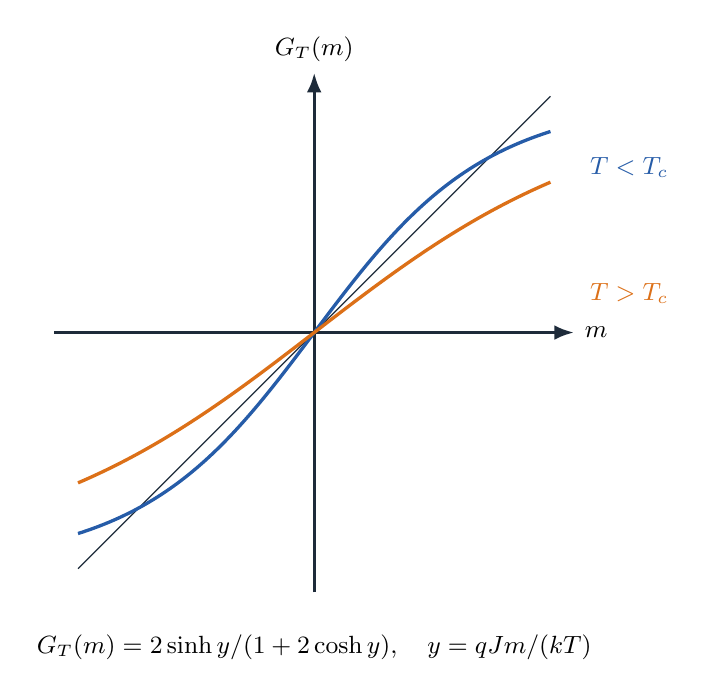
\begin{tikzpicture}[x=1cm,y=1cm,font=\small]
\draw[axis] (-3.3,0)--(3.3,0) node[right] {$m$};\draw[axis] (0,-3.3)--(0,3.3) node[above] {$G_T(m)$};\draw[ink] (-3,-3)--(3,3);\draw[blue,very thick] plot coordinates {(-3.000000,-2.552811) (-2.949580,-2.536527) (-2.899160,-2.519646) (-2.848739,-2.502148) (-2.798319,-2.484013) (-2.747899,-2.465218) (-2.697479,-2.445742) (-2.647059,-2.425564) (-2.596639,-2.404660) (-2.546218,-2.383008) (-2.495798,-2.360585) (-2.445378,-2.337367) (-2.394958,-2.313330) (-2.344538,-2.288452) (-2.294118,-2.262708) (-2.243697,-2.236075) (-2.193277,-2.208529) (-2.142857,-2.180046) (-2.092437,-2.150604) (-2.042017,-2.120179) (-1.991597,-2.088750) (-1.941176,-2.056295) (-1.890756,-2.022792) (-1.840336,-1.988221) (-1.789916,-1.952564) (-1.739496,-1.915802) (-1.689076,-1.877919) (-1.638655,-1.838899) (-1.588235,-1.798730) (-1.537815,-1.757398) (-1.487395,-1.714895) (-1.436975,-1.671213) (-1.386555,-1.626345) (-1.336134,-1.580291) (-1.285714,-1.533049) (-1.235294,-1.484621) (-1.184874,-1.435015) (-1.134454,-1.384238) (-1.084034,-1.332303) (-1.033613,-1.279225) (-0.983193,-1.225023) (-0.932773,-1.169720) (-0.882353,-1.113342) (-0.831933,-1.055920) (-0.781513,-0.997487) (-0.731092,-0.938081) (-0.680672,-0.877744) (-0.630252,-0.816520) (-0.579832,-0.754459) (-0.529412,-0.691612) (-0.478992,-0.628036) (-0.428571,-0.563789) (-0.378151,-0.498933) (-0.327731,-0.433534) (-0.277311,-0.367657) (-0.226891,-0.301373) (-0.176471,-0.234753) (-0.126050,-0.167870) (-0.075630,-0.100798) (-0.025210,-0.033612) (0.025210,0.033612) (0.075630,0.100798) (0.126050,0.167870) (0.176471,0.234753) (0.226891,0.301373) (0.277311,0.367657) (0.327731,0.433534) (0.378151,0.498933) (0.428571,0.563789) (0.478992,0.628036) (0.529412,0.691612) (0.579832,0.754459) (0.630252,0.816520) (0.680672,0.877744) (0.731092,0.938081) (0.781513,0.997487) (0.831933,1.055920) (0.882353,1.113342) (0.932773,1.169720) (0.983193,1.225023) (1.033613,1.279225) (1.084034,1.332303) (1.134454,1.384238) (1.184874,1.435015) (1.235294,1.484621) (1.285714,1.533049) (1.336134,1.580291) (1.386555,1.626345) (1.436975,1.671213) (1.487395,1.714895) (1.537815,1.757398) (1.588235,1.798730) (1.638655,1.838899) (1.689076,1.877919) (1.739496,1.915802) (1.789916,1.952564) (1.840336,1.988221) (1.890756,2.022792) (1.941176,2.056295) (1.991597,2.088750) (2.042017,2.120179) (2.092437,2.150604) (2.142857,2.180046) (2.193277,2.208529) (2.243697,2.236075) (2.294118,2.262708) (2.344538,2.288452) (2.394958,2.313330) (2.445378,2.337367) (2.495798,2.360585) (2.546218,2.383008) (2.596639,2.404660) (2.647059,2.425564) (2.697479,2.445742) (2.747899,2.465218) (2.798319,2.484013) (2.848739,2.502148) (2.899160,2.519646) (2.949580,2.536527) (3.000000,2.552811)};
\draw[orange,very thick] plot coordinates {(-3.000000,-1.909326) (-2.949580,-1.887496) (-2.899160,-1.865288) (-2.848739,-1.842701) (-2.798319,-1.819731) (-2.747899,-1.796377) (-2.697479,-1.772636) (-2.647059,-1.748505) (-2.596639,-1.723984) (-2.546218,-1.699071) (-2.495798,-1.673765) (-2.445378,-1.648064) (-2.394958,-1.621969) (-2.344538,-1.595478) (-2.294118,-1.568592) (-2.243697,-1.541310) (-2.193277,-1.513634) (-2.142857,-1.485564) (-2.092437,-1.457101) (-2.042017,-1.428248) (-1.991597,-1.399005) (-1.941176,-1.369375) (-1.890756,-1.339361) (-1.840336,-1.308966) (-1.789916,-1.278193) (-1.739496,-1.247046) (-1.689076,-1.215529) (-1.638655,-1.183648) (-1.588235,-1.151406) (-1.537815,-1.118809) (-1.487395,-1.085864) (-1.436975,-1.052576) (-1.386555,-1.018953) (-1.336134,-0.985000) (-1.285714,-0.950727) (-1.235294,-0.916141) (-1.184874,-0.881249) (-1.134454,-0.846062) (-1.084034,-0.810588) (-1.033613,-0.774837) (-0.983193,-0.738819) (-0.932773,-0.702543) (-0.882353,-0.666022) (-0.831933,-0.629265) (-0.781513,-0.592285) (-0.731092,-0.555093) (-0.680672,-0.517701) (-0.630252,-0.480121) (-0.579832,-0.442367) (-0.529412,-0.404451) (-0.478992,-0.366386) (-0.428571,-0.328186) (-0.378151,-0.289865) (-0.327731,-0.251436) (-0.277311,-0.212913) (-0.226891,-0.174310) (-0.176471,-0.135642) (-0.126050,-0.096924) (-0.075630,-0.058169) (-0.025210,-0.019392) (0.025210,0.019392) (0.075630,0.058169) (0.126050,0.096924) (0.176471,0.135642) (0.226891,0.174310) (0.277311,0.212913) (0.327731,0.251436) (0.378151,0.289865) (0.428571,0.328186) (0.478992,0.366386) (0.529412,0.404451) (0.579832,0.442367) (0.630252,0.480121) (0.680672,0.517701) (0.731092,0.555093) (0.781513,0.592285) (0.831933,0.629265) (0.882353,0.666022) (0.932773,0.702543) (0.983193,0.738819) (1.033613,0.774837) (1.084034,0.810588) (1.134454,0.846062) (1.184874,0.881249) (1.235294,0.916141) (1.285714,0.950727) (1.336134,0.985000) (1.386555,1.018953) (1.436975,1.052576) (1.487395,1.085864) (1.537815,1.118809) (1.588235,1.151406) (1.638655,1.183648) (1.689076,1.215529) (1.739496,1.247046) (1.789916,1.278193) (1.840336,1.308966) (1.890756,1.339361) (1.941176,1.369375) (1.991597,1.399005) (2.042017,1.428248) (2.092437,1.457101) (2.142857,1.485564) (2.193277,1.513634) (2.243697,1.541310) (2.294118,1.568592) (2.344538,1.595478) (2.394958,1.621969) (2.445378,1.648064) (2.495798,1.673765) (2.546218,1.699071) (2.596639,1.723984) (2.647059,1.748505) (2.697479,1.772636) (2.747899,1.796377) (2.798319,1.819731) (2.848739,1.842701) (2.899160,1.865288) (2.949580,1.887496) (3.000000,1.909326)};
\node[blue] at (4,2.1) {$T<T_c$};\node[orange] at (4,.5) {$T>T_c$};\node at (0,-4) {$G_T(m)=2\sinh y/(1+2\cosh y),\quad y=qJm/(kT)$};
\end{tikzpicture}

% 13 question-07
\begin{tikzpicture}[scale=1]
  \draw[body] (-4,0)--(4,0);
  \coordinate (O) at (-2.2,0);
  \coordinate (C) at ($(O)+(58:2.5)$);
  \coordinate (A) at ($(O)+(58:4)$);
  \draw[body,line width=3pt] (O)--(A);
  \filldraw[fill=white,body] (O) circle(3pt) node[below] {$O$};
  \fill[orange] (C) circle(3pt) node[right] {$C$};
  \draw[guide] (O)--++(0,4.2);
  \draw[blue,very thick] (O)++(90:1.2) arc[start angle=90,end angle=58,radius=1.2];
  \node[blue] at (-1.55,1.45) {$\theta$};
  \draw[dim] ($(O)+(.25,.15)$)--($(C)+(.25,.15)$) node[midway,below right] {$r_c$};
  \node[align=left,anchor=west] at (2.4,2.4) {$I_O=\lambda mr_c^2$\\杆向右倒下};
\end{tikzpicture}

% 14 solution-07
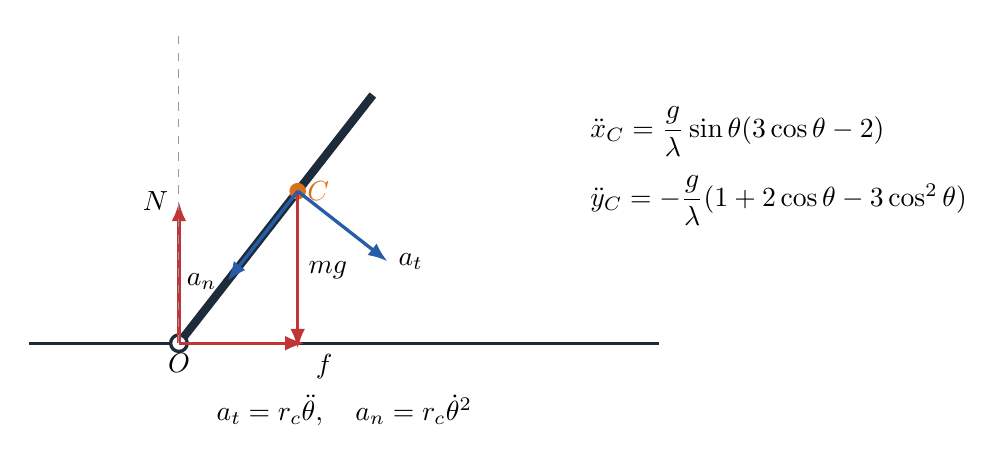
\begin{tikzpicture}[scale=1]
  \draw[body] (-4,0)--(4,0);
  \coordinate (O) at (-2.1,0); \coordinate (C) at ($(O)+(52:2.45)$);
  \coordinate (A) at ($(O)+(52:4)$);
  \draw[body,line width=3pt] (O)--(A);
  \filldraw[fill=white,body] (O) circle(3pt) node[below] {$O$};
  \fill[orange] (C) circle(3pt) node[right] {$C$};
  \draw[force] (C)--++(0,-2) node[midway,right] {$mg$};
  \draw[force] (O)--++(0,1.8) node[left] {$N$};
  \draw[force] (O)--++(1.6,0) node[below right] {$f$};
  \draw[vec] (C)--++(-38:1.45) node[right] {$a_t$};
  \draw[vec] (C)--++(232:1.45) node[left] {$a_n$};
  \draw[guide] (O)--++(0,4);
  \node[align=left,anchor=west] at (3,2.25)
   {$\ddot x_C=\dfrac g\lambda\sin\theta(3\cos\theta-2)$\\[6pt]
    $\ddot y_C=-\dfrac g\lambda(1+2\cos\theta-3\cos^2\theta)$};
\node at (0,-.85) {$a_t=r_c\ddot\theta,\quad a_n=r_c\dot\theta^2$};
\end{tikzpicture}

% 15 question-08
\begin{tikzpicture}[scale=.95]
  \draw[body] (-5,-2)--(5,-2);
  \coordinate (O) at (0,0);
  \draw[body,line width=2pt] (O) circle(2);
  \fill[ink] (O) circle(2pt) node[above right] {$O$};
  \coordinate (P) at ($(O)+(-125:2)$);
  \filldraw[fill=orange!25,body] (P) circle(.19) node[left] {$P(m,q)$};
  \draw[orange,very thick] (O)--(P);
  \draw[guide] (O)--++(0,-2);
  \draw[blue,very thick] (O)++(-90:.85) arc[start angle=-90,end angle=-125,radius=.85];
  \node[blue] at (-.7,-.95) {$\beta$};
  \draw[axis] (0,2.65)--(2.4,2.65) node[right] {$x$};
  \node at (3.2,.9) {$\otimes\ B$};
  \draw[orange,very thick,-{Latex}] (2.2,0) arc[start angle=0,end angle=-75,radius=2.2];
  \node[orange] at (2.55,-.9) {纯滚动};
\end{tikzpicture}

% 16 solution-08
\begin{tikzpicture}[scale=.92]
  \draw[body] (-5,-2)--(5,-2);
  \coordinate (O) at (0,0); \draw[body,line width=2pt] (O) circle(2);
  \coordinate (P) at ($(O)+(-135:2)$);
  \fill[ink] (O) circle(2pt) node[above right] {$O$};
  \filldraw[fill=orange!25,body] (P) circle(.2) node[left] {$P$};
  \draw[orange,very thick] (O)--(P);
  \draw[vec] (O)--++(2.1,0) node[above] {$\dot x$};
  \draw[vec] (P)--++(1.55,0) node[below right] {$\dot x$};
  \draw[vec] (P)--++(-45:1.65) node[above right] {$r\dot\beta$};
  \draw[force] (P)--++(-1.25,0) node[left] {$F_{Bx}$};
  \node at (2.7,-.45) {$\otimes\ B$};
  \draw[guide] (O)--++(0,-2);
  \node[align=left,anchor=west] at (3.1,1.25)
   {$\dot x_P=\dot x-r\dot\beta\cos\beta$\\[5pt]
    $\dot y_P=r\dot\beta\sin\beta$\\[5pt]
    $\omega_{\rm rel}=\dot\beta-\dot x/r$\\相对静止：$r\dot\beta=\dot x$};
  \node at (0,-3.6) {$3\dot x-r\dot\beta\cos\beta=(qBr/m)\cos\beta$};
\end{tikzpicture}
\end{document}
